\documentclass[french]{article}

\usepackage[french]{babel}

\usepackage[hidelinks,unicode]{hyperref}
\usepackage[dvipsnames]{xcolor}
\usepackage{graphicx}
\usepackage{amsmath}
\usepackage[left=1.3in,right=1.3in]{geometry}
\usepackage{microtype}
\usepackage{upquote}
\usepackage{csquotes}
\usepackage{url}
\usepackage[backend=biber]{biblatex}
\usepackage{marvosym}

\usepackage{tikz}
\usepackage{fontspec}

\usepackage{minted}
%\usemintedstyle{colorful}

\usepackage{pdfpages}

\usepackage{titling}
\newcommand{\subtitle}[1]{%
  \posttitle{%
    \par\end{center}
    \begin{center}\large#1\end{center}
    \vskip0.5em}%
}

\addbibresource{references.bib}

\title{Martine résout le problème du voyageur de commerce}
\subtitle{Avec un algorithme A*}
\author{Maxence \textsc{Aïci} \and Rémi \textsc{Nicole}}

\begin{document}

\maketitle

\tableofcontents

\part{Modélisation}

\paragraph{} Le problème du voyageur de commerce est probablement le problème
NP-complet le plus connu en algorithmique, mais dans le doute, voici la
définition de Wikipédia~\cite{wiki:tsp}:

\begin{quote}
	``Given a list of cities and the distances between each
	pair of cities, what is the shortest possible route that visits each city
	exactly once and returns to the origin city?''
\end{quote}

\paragraph{} Quant aux algorithmes de type A*, il s'agit tout simplement d'une
amélioration de l'algorithme de Dijkstra qui choisit sans aucun scrupule les
sommets qui sont les plus susceptibles de nous mener à la solution optimale. On
calcule cette ``susceptibilité'' grâce à une heuristique qui calculera de
manière arbitraire une estimation du score restant pour aller à l'arrivée.

De manière mathématique, parce qu'en algorithmique, on aime bien écrire des
équations compliquées, et en plus en \LaTeX, ça nous donne un rendu magnifique:

\[f(n) = g(n) + h(n)\]

Avec:
\begin{itemize}
	\item $n$ l'étape par laquelle l'algorithme suggère de passer
	\item $f(n)$ l'estimation du coût total en passant par l'étape $n$
	\item $g(n)$ le coût d'aller du début jusqu'à l'étape $n$
	\item $h(n)$ l'estimation du coût pour aller de l'étape $n$ à l'arrivée
\end{itemize}

\section{Graphe de résolution de problème}

\paragraph{} Tout d'abords, il nous faut un arbre de résolution de problème
pour pouvoir faire de l'A*. Nous le définissons donc ainsi:

Si la carte des villes ressemble à ceci:
\begin{center}
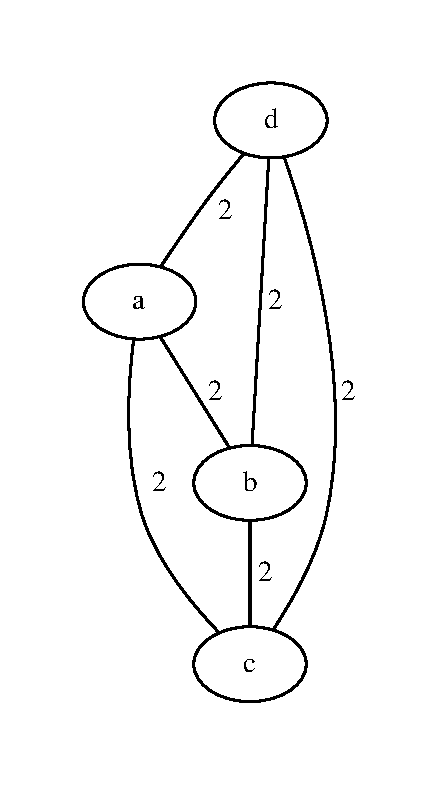
\includegraphics[scale=0.5]{graphs/modeling-the-problem_example1-map.pdf}
\end{center}

Alors on aura notre graphe de résolution de problème, ou PSG pour l'acronyme
anglais (aucune affiliation avec aucun groupe sportif), qui sera:
\begin{center}
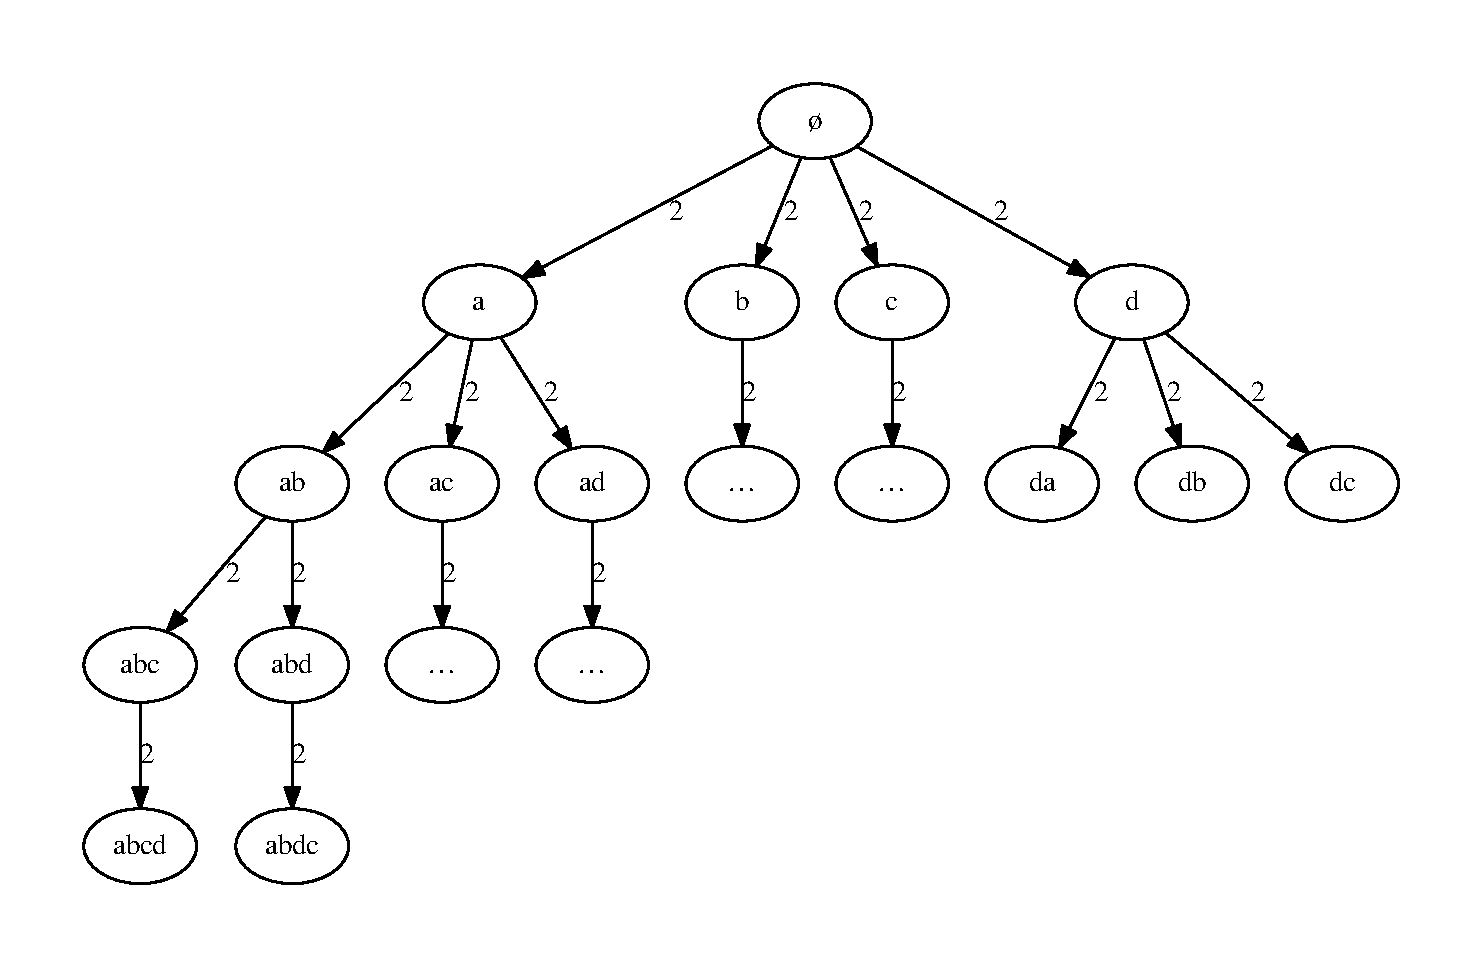
\includegraphics[scale=0.5]{graphs/modeling-the-problem_example1-psg.pdf}
\end{center}

Et, par exemple, après avoir pris le chemin A $\rightarrow$ B $\rightarrow$ C,
on aura:
\begin{center}
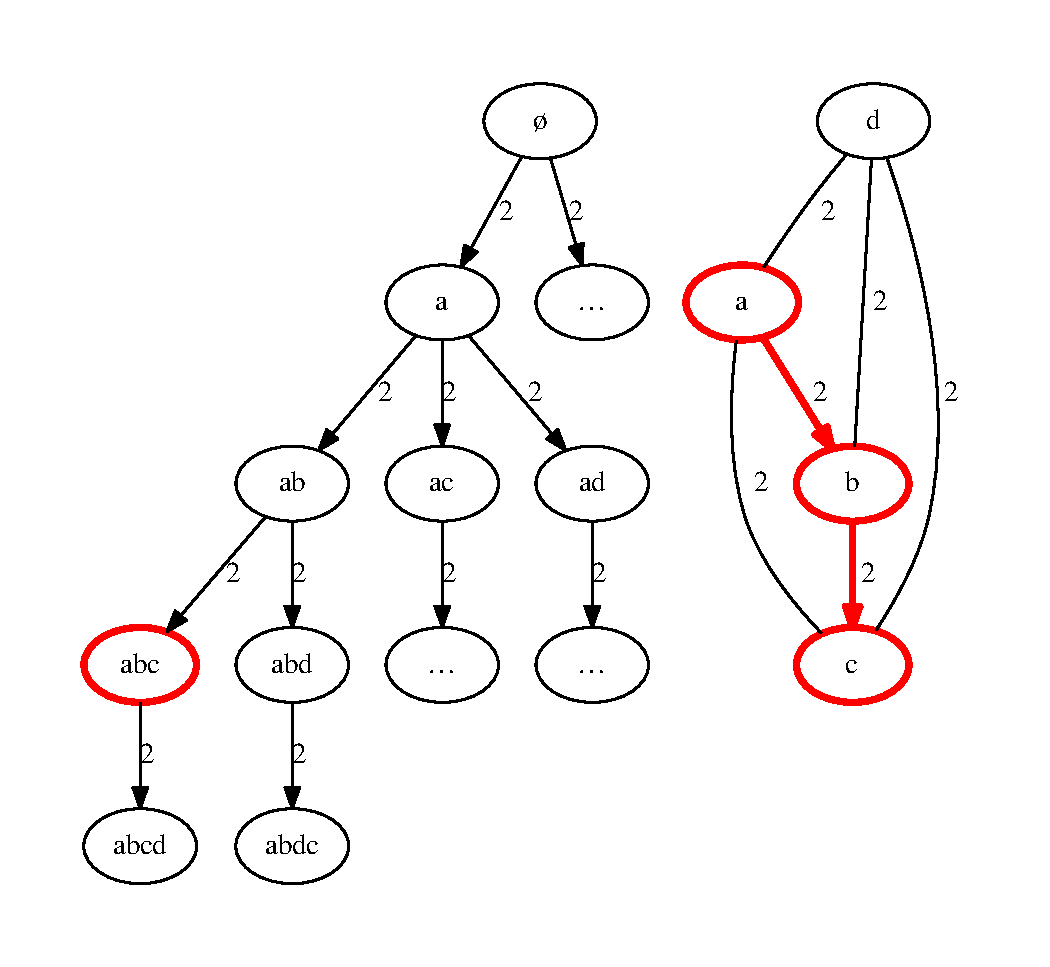
\includegraphics[scale=0.5]{graphs/modeling-the-problem_example2.pdf}
\end{center}

\section{Heuristiques}

\paragraph{} Pour ne pas être aussi inefficace que Dijkstra et pouvoir enfin
s'appeler A*, parce qu'avoir un nom prononçable c'est aussi important, il nous
faut des heuristiques. Il est aussi important d'avoir des heuristiques qui
estiment suffisamment bien le poids du chemin restant, mais tout en restant
facile à calculer parce que l'on risque d'en avoir souvent besoin au cours de
l'algorithme.

\subsection{Nulle}

\paragraph{} Comme son nom l'indique, l'heuristique nulle n'est pas terrible.
Il s'agit tout simplement de l'heuristique qui n'estime pas. En dehors d'être
le Saint Graal des heuristiques pour programmeurs fainéants, elle nous servira
aussi à tester notre algorithme, qui se ramènera donc à Dijkstra, ce qui m'a
fait reprendre à trois fois avant de pouvoir taper ce nom correctement. À
n'utiliser qu'en derniers recours, donc.

\subsection{Arête de poids minimum}

\paragraph{} Une autre heuristique simple, mais pas autant que précédemment,
est de prendre l'arête de poids minimum dans la carte privée des villes
parcourues, et de le multiplier par le nombre de villes restant à parcourir. Ce
n'est pas vraiment une bonne approximation, mais au moins on est sûr que le
chemin optimal aura comme borne inférieure le résultat de cette heuristique.

\subsection{Dijkstra}

\paragraph{} Curieuse coïncidence, on peut utiliser Dijsktra dans une
heuristique A*. Cette heuristique consiste à prendre le plus cours chemin de la
ville actuelle jusqu'à la ville de départ. Avec un peu de chance cette
approximation sera exacte, même si la complexité laisse à désirer.

\subsection{Arbre de poids minimum}

\paragraph{} Une utilisation intéressante de l'arbre de poids minimum, ou MST
pour l'acronyme anglais que l'on ne commentera pas, est de l'intégrer dans une
heuristique du voyageur de commerce. De plus, si l'on fait les bons choix
d'implémentation, il a une complexité de:

\[O(|\text{arêtes}| \times \log\left(|\text{sommets}|\right))\]

ce qui pourrait être un bon compromis entre la précision de l'approximation et
la complexité de l'heuristique.

Une fois que le MST de la carte, toujours privée des villes déjà parcourues,
est obtenu, il nous suffira de sommer le poids des arêtes et on aura notre
approximation!

\part{Outils}

\section{Moteur de production}

\begin{itemize}
	\item Meson~\cite{tools:meson} todo: dire que le site est moche
	\item Ninja~\cite{tools:ninja}
\end{itemize}

\textbf{\Huge{TODO}}

\section{Débogage}

\begin{itemize}
	\item gdb
	\item valgrind
	\item gprof
	\item Kcachegrind
\end{itemize}

\textbf{\Huge{TODO}}

\part{Implémentation des structures}

\paragraph{} Afin d'implémenter (ou d'implanter pour les gens bizarres) ces
types de graphes nous avons décidés de reprendre ce que j'avais\footnote{Ici
	Rémi qui parle} fait en C++ pour implémenter des algorithmes de l'unité
IT-3004 mais avait abandonnée au bout de deux jours parce que flemmingite
aigüe.

Nous avons donc développé par-dessus un bout de code en C++ développé sur un
coup de tête, sans réflexion au préalable, et abandonné très rapidement. Aucun
moyen que cela tourne mal, donc.

\paragraph{} Il est important de préciser qu'au tout début du projet, nous
avions décidé d'utiliser la BGL (Boost Graph Library) pour implémenter par
dessus l'algorithme A*. Cependant, après beaucoup de frustration, de cheveux
perdus, et après avoir remarqué le manque de documentation, tutoriels ou
ressources en ligne, il était évident que ce serait une chose à ne plus
refaire.

\section{État initial}

\subsection{Philosophie}

\paragraph{} Au tout début du projet, la partie graphe était seulement composée
de 4 classes: le graphe représenté par une liste d'adjacence, le graphe
représenté par une matrice d'adjacence, et leur classe ``d'itérateur évolué''
sur les sommets. Tous les graphes étaient orientés (et ils le sont toujours,
d'ailleurs)

\paragraph{} La classe de graphe représenté par une liste d'adjacence était
dans le namespace \texttt{list} et la classe de graphe représenté par une
matrice d'adjacence était dans le namespace \texttt{matrix}. L'idée était de
pouvoir faire:

\begin{minted}{cpp}
	using list::Graph;
	using list::Node;
	Graph myGraph;
\end{minted}

Ou l'équivalent avec \texttt{matrix} pour pouvoir choisir son type
d'implémentation. Même si, après rétrospection, ce n'était peut-être pas le
meilleur choix, cette philosophie est restée et a un peu évoluée au cours du
projet.

\subsection{Fonctionnalités}

\paragraph{} Au début du projet, voici ce qu'il était possibles de faire:

\begin{itemize}
	\item Construire un graphe directement avec une liste d'arcs:
		\begin{minted}{cpp}
	Graph myGraph{{1, 2}, {3, 4}, {1, 3}};
	Graph myGraph(4, {1, 2}, {3, 4}, {1, 3});
		\end{minted}
{\fontspec{Humor-Sans}
	\begin{tikzpicture}[overlay]
		\draw[thick,<-] (6:4.3) to [out=-30,in=180] (-2:8) [anchor=west,text width=6cm] node{Nombre de sommets\\ {\color{red} parametre disparu}};
	\end{tikzpicture}
}
	\item Ajouter des arcs.
	\item Calculer le symétrique du graphe.
	\item Calculer un composant connexe / fortement connexe du graphe.
	\item Compter le nombre d'arcs / de sommets.
	\item Opérer sur des connexions entre sommets:
		\begin{minted}{cpp}
	myGraph[1].isConnectedTo(3);
	myGraph[2].connectTo(4);
	myGraph[3].disconnectFrom(4);
		\end{minted}
\end{itemize}

\section{Évolutions}

\paragraph{} Il ne s'agit pas ici de parler de Pokémon, mais bien de
l'évolution du projet sur la partie implémentation des structures de graphes.
Quel dommage\ldots

\subsection{Refactorisations}

\paragraph{} Le projet a donc commencé de manière très agréable avec une série
de refactorisation du code de ce projet, afin de lui permettre d'être utilisée
pour faire des ``vrais'' algorithmes par-dessus.

\paragraph{} Nous avons d'abords mis certaines fonctions hors des classes car
elles ne méritaient pas le statut de ``méthodes''. Il s'agit surtout
d'algorithmes qui opèrent sur le graphe, comme le calcul de symétrique ou de
composantes connexes.

Afin de facilité le portage de ces fonctions et le développement de futurs
algorithmes, nous avons aussi rajouté des méthodes de parcours de sommets,
arcs, adjacents. Ces fonctions prennent en paramètre une fonction de rappel,
autrement appelé \emph{lambda} en C++, ce qui nous permets d'avoir un code
source clair et très joli à observer. Par exemple, pour l'algorithme du calcul
du symétrique, cela se résume à 4 lignes et un tiers:

\begin{listing}[H]
\begin{minted}{cpp}
Graph symmetric(Graph const& g) {
	Graph symmetricGraph;

	g.eachEdges([&symmetricGraph, &g](Node begin, Node end) {
		symmetricGraph.addEdges({end.getId(), begin.getId()});
	});

	return symmetricGraph;
}
\end{minted}
\caption{Un extrait de code aussi clair que net et précis}
\label{tsp:symmetric}
\end{listing}

\paragraph{} L'étape suivante a été de rajouter le type \texttt{ConstNode} qui,
à l'instar de la class \texttt{Node} permet d'accéder à des méthodes sur les
sommets uniquement, mais à partir d'un \texttt{Graph} non modifiable
(\mintinline{cpp}{const}). Pour éviter la duplication de code entre
\texttt{Node} et \texttt{ConstNode}, la solution choisie a été de créer une
classe mère \texttt{GenericNode} ayant un template pour pouvoir choisir si le
type des connexions internes est une référence ou une référence constante,
parce que \textbf{C++}!

\paragraph{} Puis, comme tout programmeur se doit de respecter les conventions
du langage, nous avons mis toutes les classe dans un namespace créé
spécialement pour l'occasion, que nous avons appelé \texttt{graph}, reflétant
notre nature d'adolescent engloutis par la société de consommation, délaissé
sans aucune originalité propre.

\paragraph{} Ensuite viens la plus grosse et donc la plus horrible des
refactorisations qui a été de permettre de pouvoir stocker des valeurs d'un
types arbitraires pour chaque sommet et pour chaque arc. Il a donc fallu
rajouter un double template aux classes \texttt{Graph}. Nous avons choisi de
stocker ce que l'on appellera les propriétés dans un vecteur pour les sommets,
et dans une map ayant pour clef une paire d'identifiant dans le cas des arcs.
Il a fallu ensuite concevoir une interface digne de ce nom. Nous avons aussi
fournis des structures pour des graphes avec des fonctionnalités basiques,
comme un poids ou, comme par hasard, des propriétés propre à l'A* ($g(n)$,
$h(n)$).

\paragraph{} Enfin, il a fallu permettre d'utiliser les Graphes avec des
chaînes de caractères pour que cela soit plus clair pour le nom des villes. Il
a donc été nécessaire de remplacer l'utilisation d'identifiant, qui possédaient
le type \mintinline{cpp}{size_t}, par des \mintinline{cpp}{std::string}. Ça a
été le cas par exemple pour la map des propriétés des arcs.

\subsection{Trucs sympa}

\paragraph{} Même s'il y a eu beaucoup de refactorisation et beaucoup de
messages d'erreurs incompréhensibles (ce qui est quasiment la philosophie du
C++), il y avait quand même du bon dans ce sous-projet. En voici un top trois:

\subsubsection{3\ieme{} place}

\paragraph{} Les tests unitaires couvrent 97.8\% de la base de code! \Smiley{}

\subsubsection{2\ieme{} place}

\paragraph{} Il est possible d'afficher n'importe quel graphe sous la forme de
digraph Graphviz. De plus, si les arcs sont pondérés, le poids s'affiche à côté
des arcs.

\subsubsection{1\iere{} place}

\paragraph{} Il est possible de créer un Graphe directement en décrivant ses
arcs avec leur(s) propriété(s). Cela a nécessité d'outrepasser le fait que le
constructeur d'un tuple ayant pour paramètre une
\mintinline{cpp}{std::initializer_list} est explicite, pour pouvoir remplacer
ceci:

\begin{listing}[H]
\begin{minted}{cpp}
Graph myGraph{
	std::make_tuple("Paris", "New-York", WeightedProperty{5851}),
	std::make_tuple("New-York", "Paris", WeightedProperty{5851}),
	std::make_tuple("Houilles", "Noisy-Champs", WeightedProperty{13}),
	std::make_tuple("Noisy-Champs", "Houilles", WeightedProperty{13})
};
\end{minted}
\caption{Beuh}
\label{tsp:beuh}
\end{listing}

Par ceci:

\begin{listing}[H]
\begin{minted}{cpp}
Graph myGraph{{"Paris", "New-York", {5851}},
              {"New-York", "Paris", {5851}},
              {"Houilles", "Noisy-Champs", {13}},
              {"Noisy-Champs", "Houilles", {13}}};
\end{minted}
\caption{Beaucoup mieux!}
\label{tsp:better}
\end{listing}

\part{Implémentation de l'algorithme}

\paragraph{} Après avoir passé une semaine entière à développer une
bibliothèque complètement superflue pour l'algorithme A* et autre algorithmes
graphesques, nous avons décidé de nous attaquer enfin à l'implémentation du
cœur du projet PR-3602.

\paragraph{} Afin d'enfin nous détacher de cette horrible masse de
conformistes, nous avons choisir d'utiliser cette fois si le namespace
\texttt{awesome} pour englober notre implémentation. Nous avons aussi décidé de
démarrer notre propre mouvement contre-culture. Cependant, nous avons un doute
sur l'efficacité de notre implémentation de la dernière proposition.

\section{Les heuristiques}

\paragraph{} Comme la clarté du code est un critère extrêmement important pour
cette unité, nous avons créé une classe abstraite \texttt{Heuristique} (de
nouveau dans l'inoriginalité). Cette classe a besoin d'un référence vers le PSG
et une référence à la carte de base à la construction, et possède une fonction
virtuelle pure \mintinline{cpp}{operator()} prenant en paramètre l'état actuel
(la carte privée des villes déjà parcourues) et le sommets sur lequel on est
dans le graph de résolution.

\subsection{Nulle}

\paragraph{} Il n'y a pas grand chose à dire ici. Voici la surcharge de
\mintinline{cpp}{operator()} pour référence seulement:

\begin{listing}[H]
\begin{minted}{cpp}
int NullHeuristic::operator()(MapGraph const&, GraphConstNode const&) {
	return 0;
}
\end{minted}
\caption{Une fonction très compliquée}
\label{tsp:nulloperator}
\end{listing}

\subsection{Arête de poids minimum}

\paragraph{} Aussi très simple à coder, nous avons utilisé une combinaison d'un
algorithme de calcul de minimum avec la méthode \texttt{eachEdges}.

\subsection{Dijkstra}

\paragraph{} Oups, nous avons oublié de l'implémenter. Ce n'est pas très grave
parce que de toute manière la complexité de cette heuristique est trop élevée,
ou tout autre excuse fournie allègrement par le biais de confirmation ou dénis
scientifique.

\subsection{Arbre de poids minimum}

\paragraph{} Ayant pris l'algorithme directement depuis un certain polycopié de
couleur saumon, le plus difficile dans cette heuristique a sûrement été de
remarquer que nous essayions de faire marcher l'algorithme de Prim sur un graph
orienté.

Cet ainsi qu'est né la fonction \texttt{undirected} calculant le graph
non-orienté équivalent, tout comme la fonction \texttt{minimumSpanningTree}
d'ailleurs.

\section{Le solutionneur (enfin)}

\subsection{Types}

\paragraph{} Étant dans l'obligation de traduire tous les concepts anglais,
nous sommes (regrettablement) obligé de mettre ``solutionneur'' à la place du
simple et beau mot anglais: ``solver''.

\paragraph{} Nous avons donc utilisé deux types de graphes sur lequel
travaillé, avec des propriétés gentiment fournies par notre bibliothèque:

\begin{listing}[H]
\begin{minted}{cpp}
using MapGraph = Graph<NoProperty, WeightedProperty>;
\end{minted}
\caption{Type utilisé pour la carte}
\label{tsp:map}
\end{listing}

\begin{listing}[H]
\begin{minted}{cpp}
using PSGGraph = Graph<AstarNodeProperty<MapGraph>, WeightedProperty>;
\end{minted}
\caption{Type utilisé pour notre graphe de résolution de problème}
\label{tsp:psg}
\end{listing}

\paragraph{} Avec ci-dessous les déclarations de \texttt{NoProperty},
\texttt{WeightedProperty}, \texttt{AstarNodeProperty}:

\begin{listing}[H]
\begin{minted}{cpp}
struct NoProperty {
	bool operator==(NoProperty const&) const {
		return true;
	}
};
\end{minted}
\caption{Déclaration de la structure NoProperty}
\label{tsp:noprop}
\end{listing}

\begin{listing}[H]
\begin{minted}{cpp}
struct WeightedProperty {
	int weight;

	bool operator==(WeightedProperty const& other) const {
		return weight == other.weight;
	}
};
\end{minted}
\caption{Déclaration de la structure WeightedProperty}
\label{tsp:weightedprop}
\end{listing}

\begin{listing}[H]
\begin{minted}{cpp}
template <typename State>
struct AstarNodeProperty {
	int gScore;
	int hScore;

	State state;

	bool operator==(AstarNodeProperty const& other) const;
};

template <>
struct AstarNodeProperty<void> {
	int gScore;
	int hScore;

	bool operator==(AstarNodeProperty const& other) const;
};
\end{minted}
\caption{Déclaration de la structure AstarNodeProperty}
\label{tsp:astarnodeprop}
\end{listing}

\paragraph{} Il nous a semblé intéressant de pouvoir mettre l'état
intermédiaire dans chaque sommet, pour qu'il puisse être utilisable rapidement
dans les heuristiques. Si jamais l'utilisateur ne veut pas stocker l'état
intermédiaire, c'est à ça que sert la spécialisation avec
\mintinline{cpp}{void}. Mais pour cela il faudra qu'un utilisateur existe.

\subsection{Structure}

{\fontspec{Humor-Sans} \paragraph{} La structure de la classe TSPSolver...}
oups, pardon, mauvaise police de caractère. Je disais donc que la structure de
la classe TSPSolver comporte 8 méthodes:

\begin{itemize}
	\item Le constructeur (prends en paramètre la carte de base)
	\item \texttt{goForIt}, qui lance l'algorithme
	\item \texttt{finishLine}, qui reconstruit le chemin de villes un fois l'algorithme terminé
	\item \texttt{develop}, qui développe un sommet du PSG
	\item \texttt{findInOpenNodes}, qui retourne un itérateur d'un sommet sur
		la liste OUVERT (je sais pas pourquoi il faut le mettre en majuscule
		mais c'était sur le site PR-3602).
	\item \texttt{isGoal}, bah ça vérifie si un sommet est du PSG est un but.
	\item \texttt{isFailure} pareil que précédemment mais dans le cas d'une
		impossibilité (si l'on retourne à la ville de départ sans être passé
		par toutes les villes)
	\item \texttt{isStart} vérifie si un sommet du PSG ne contient que la ville
		de départ.
	\item \mintinline{cpp}{CompareFunc::operator()} compare deux sommets du PSG
		relativement au $f(n) = g(n) + h(n)$
\end{itemize}

\paragraph{} ``Il y a 9 méthodes!'' vous empresserez vous de me dire, désireux
de pointer chaque erreurs de ce rapport. Cependant, tout était prévu: le
constructeur n'est pas une ``vraie'' méthode, ni
\mintinline{cpp}{CompareFunc::operator()} qui est dans une structure interne à
la classe. Chacun compte donc pour $\frac{1}{2}$.

\paragraph{} À ce propos, il me semble judicieux d'expliquer la raison de
l'existence de la structure \texttt{CompareFunc}. Plutôt que de chercher le
sommet du PSG ayant le score $f(n)$ minimal parmi tous les sommets de la liste
\textbf{OUVERT}, nous avons décidé d'utiliser un conteneur stockant de manière
triée, permettant une insertion et recherche de complexité logarithmique. La
définition de la liste \textbf{\Large{OUVERT}} est telle:

\begin{minted}{cpp}
std::multiset<GraphConstNode, CompareFunc> openNodes;
\end{minted}

\paragraph{} Il s'agit d'un \texttt{multiset} et non un \texttt{set} car aux
yeux de ces classes, si l'on fourni notre fonction de comparaison, deux sommets
ayant le même score $f(n)$ sont égaux. Il nous faut donc un conteneur
permettant de stocker plusieurs sommets ``égaux'', donc \texttt{multiset}.

\paragraph{} Tout le reste s'est passé très vite. Prendre le premier élément de
la liste \textbf{\huge{OUVERT}}, développer le sommet, ce qui reviens à
regarder les adjacents du sommet actuel dans la carte intermédiaire, les
ajouter dans le PSG et la liste \textbf{\Huge{OUVERT}} s'il ne sont pas
``impossibles'', en prenant en compte leur score $g(n)$ et $h(n)$ et la
nouvelle carte intermédiaire. Il est important de noter qu'il ne faut pas
supprimer la ville de départ dans les débuts de l'algorithme, sinon le pauvre
voyageur de commerce errera éternellement entre les sommets du PSG, sans
arrivée.

\part{Tests}

\paragraph{} Après avoir passé un peu plus d'un jour à faire l'algorithme A*,
nous nous retrouvions soudainement dans cette oisiveté insoutenable.

\section{MapGen}

\section{Benchmarks}

\begin{figure}[H]
	\centering
	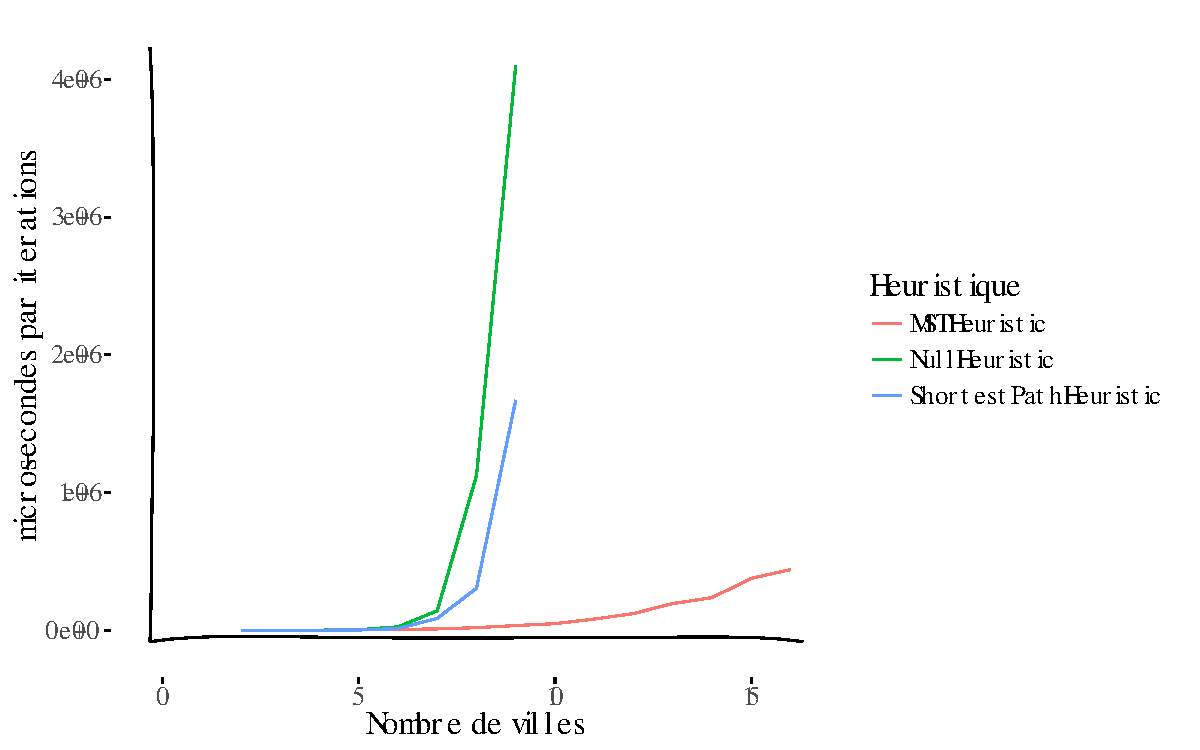
\includegraphics[scale=0.8]{graphs/benchmarks.pdf}
	\caption{Résultats du benchmark}
	\label{fig:benchmarks}
\end{figure}

\part{Jouons à Hercule Poirot}

{\Huge TODO}

cite fizzbuzz\\
gprof, kcachegrind (screenshots?)

\part{Pour aller plus loin}

{\Huge TODO}

generic astar solver

\printbibliography%

\end{document}
